% =====================================================================
% TECHNICAL GUIDE: AVEVA PROCESS SIMULATION + PYTHON REAL-TIME BRIDGE
% Author: Ezequiel Jose Valencia Urbina
% University of Brasilia (UnB) - Mechanical Systems Dynamics
% =====================================================================
\documentclass[11pt, letterpaper]{article}

\usepackage[utf8]{inputenc}
\usepackage[T1]{fontenc}
\usepackage[english]{babel}
% lmodern removed - using default CM fonts
\usepackage[margin=2.5cm, bottom=3cm, top=3cm]{geometry}
\usepackage{xcolor}
\usepackage{colortbl}
\usepackage{graphicx}
\usepackage{fancyhdr}
\usepackage{titlesec}
\usepackage{booktabs}
\usepackage{enumitem}
\usepackage{helvet}
\usepackage{float}
\usepackage{caption}
\usepackage{array}
\usepackage{multirow}
\usepackage{longtable}
\usepackage{tabularx}
\usepackage{amsmath}
\usepackage{amssymb}
\renewcommand{\familydefault}{\sfdefault}

\usepackage{tikz}
\usetikzlibrary{shapes.geometric, shapes.symbols, arrows.meta, positioning,
                fit, backgrounds, calc, shadows.blur, decorations.pathreplacing,
                chains, scopes}

\usepackage{listings}
\usepackage[most]{tcolorbox}

% =====================================================================
% COLOR PALETTE
% =====================================================================
\definecolor{avevaPurple}{HTML}{3A1041}
\definecolor{avevaMagenta}{HTML}{9B26B6}
\definecolor{avevaCyan}{HTML}{00D1FF}
\definecolor{avevaGray}{HTML}{4A4A4A}
\definecolor{avevaLight}{HTML}{F5F0F7}
\definecolor{tipGreen}{HTML}{2E7D32}
\definecolor{tipBg}{HTML}{E8F5E9}
\definecolor{warnRed}{HTML}{C62828}
\definecolor{warnBg}{HTML}{FFEBEE}
\definecolor{noteBlue}{HTML}{1565C0}
\definecolor{noteBg}{HTML}{E3F2FD}
\definecolor{diagOrange}{HTML}{E65100}
\definecolor{diagBg}{HTML}{FFF3E0}
\definecolor{codeBg}{HTML}{F8F8F8}
\definecolor{codeKeyword}{HTML}{0033B3}
\definecolor{codeComment}{HTML}{8C8C8C}
\definecolor{codeString}{HTML}{067D17}
\definecolor{stepBlue}{HTML}{1976D2}
\definecolor{stepBg}{HTML}{E8EAF6}

\usepackage[colorlinks=true, linkcolor=avevaPurple,
            urlcolor=avevaMagenta, citecolor=avevaPurple]{hyperref}

% =====================================================================
% HEADER AND FOOTER
% =====================================================================
\pagestyle{fancy}
\fancyhf{}
\renewcommand{\headrulewidth}{0.4pt}
\renewcommand{\footrulewidth}{0.4pt}
\fancyhead[L]{\textcolor{avevaPurple}{\textbf{Digital Twin Integration Guide}}}
\fancyhead[R]{\textcolor{avevaPurple}{AVEVA Process Simulation}}
\fancyfoot[L]{\textbf{\textcolor{avevaPurple}{UDP + simcentralconnect}}}
\fancyfoot[C]{\thepage}
\fancyfoot[R]{\textcolor{avevaPurple}{E. Valencia Urbina}}

% =====================================================================
% TITLE AND BOX STYLES
% =====================================================================
\titleformat{\section}{\color{avevaPurple}\normalfont\Large\bfseries}{\thesection}{1em}{}
\titleformat{\subsection}{\color{avevaMagenta}\normalfont\large\bfseries}{\thesubsection}{1em}{}
\titleformat{\subsubsection}{\color{avevaGray}\normalfont\normalsize\bfseries}{\thesubsubsection}{1em}{}

\newtcolorbox{tipbox}[1][]{enhanced, breakable, colback=tipBg, colframe=tipGreen,
  fonttitle=\bfseries\color{white}, coltitle=white,
  title={\raisebox{-1pt}{$\bigstar$}~ENGINEERING TIP}, arc=2mm, boxrule=0.6pt,
  left=3mm, right=3mm, top=2mm, bottom=2mm, #1}

\newtcolorbox{warnbox}[1][]{enhanced, breakable, colback=warnBg, colframe=warnRed,
  fonttitle=\bfseries\color{white}, coltitle=white,
  title={$\triangle$~CRITICAL WARNING}, arc=2mm, boxrule=0.6pt,
  left=3mm, right=3mm, top=2mm, bottom=2mm, #1}

\newtcolorbox{notebox}[1][]{enhanced, breakable, colback=noteBg, colframe=noteBlue,
  fonttitle=\bfseries\color{white}, coltitle=white,
  title={$\oplus$~TECHNICAL NOTE}, arc=2mm, boxrule=0.6pt,
  left=3mm, right=3mm, top=2mm, bottom=2mm, #1}

\newtcolorbox{diagbox}[1][]{enhanced, breakable, colback=diagBg, colframe=diagOrange,
  fonttitle=\bfseries\color{white}, coltitle=white,
  title={$\oslash$~TROUBLESHOOTING}, arc=2mm, boxrule=0.6pt,
  left=3mm, right=3mm, top=2mm, bottom=2mm, #1}

\newtcolorbox{goodbox}[1][]{enhanced, breakable, colback=avevaLight, colframe=avevaPurple,
  fonttitle=\bfseries\color{white}, coltitle=white,
  title={$\diamond$~INDUSTRY BEST PRACTICE}, arc=2mm, boxrule=0.6pt,
  left=3mm, right=3mm, top=2mm, bottom=2mm, #1}

\newtcolorbox{stepbox}[2][]{enhanced, breakable, colback=stepBg, colframe=stepBlue,
  fonttitle=\bfseries\color{white}, coltitle=white,
  title={STEP #2}, arc=2mm, boxrule=0.6pt,
  left=3mm, right=3mm, top=2mm, bottom=2mm, #1}

% =====================================================================
% CODE LISTING STYLES
% =====================================================================
\lstdefinestyle{csharpstyle}{
    backgroundcolor=\color{codeBg}, commentstyle=\color{codeComment}\itshape,
    keywordstyle=\color{codeKeyword}\bfseries, stringstyle=\color{codeString},
    basicstyle=\ttfamily\scriptsize, breakatwhitespace=false, breaklines=true,
    captionpos=b, keepspaces=true, numbers=left, numbersep=8pt,
    numberstyle=\tiny\color{avevaGray}, showspaces=false, showstringspaces=false,
    showtabs=false, tabsize=4, frame=single, rulecolor=\color{avevaPurple},
    language=[Sharp]C,
    morekeywords={string, var, out, async, await, nameof, double, bool, int, object}
}
\lstdefinestyle{pythonstyle}{
    backgroundcolor=\color{codeBg}, commentstyle=\color{codeComment}\itshape,
    keywordstyle=\color{codeKeyword}\bfseries, stringstyle=\color{codeString},
    basicstyle=\ttfamily\scriptsize, breakatwhitespace=false, breaklines=true,
    captionpos=b, keepspaces=true, numbers=left, numbersep=8pt,
    numberstyle=\tiny\color{avevaGray}, showspaces=false, showstringspaces=false,
    showtabs=false, tabsize=4, frame=single, rulecolor=\color{avevaPurple},
    language=Python
}


\setlength{\headheight}{15pt}

\begin{document}
\begin{titlepage}
\centering
\vspace*{0.6cm}
{\large\textcolor{avevaGray}{\textsc{Practical Engineering Guide}}\par}
\vspace{0.5cm}
{\color{avevaPurple}\rule{\textwidth}{2.5pt}}
\vspace{1cm}
{\fontsize{27}{32}\selectfont\bfseries\textcolor{avevaPurple}{Automated Dynamic Experiments\\with AVEVA Process Simulation}\par}
\vspace{0.7cm}
{\Large\bfseries\textcolor{avevaMagenta}{Custom EETK DLL, UDP Communication\\and Python with simcentralconnect}\par}
\vspace{0.8cm}
{\normalsize A reusable workflow for defining process variables, building the communication DLL, exchanging commands and measurements, and automating simulation runs and snapshot restoration.\par}
\vspace{0.9cm}
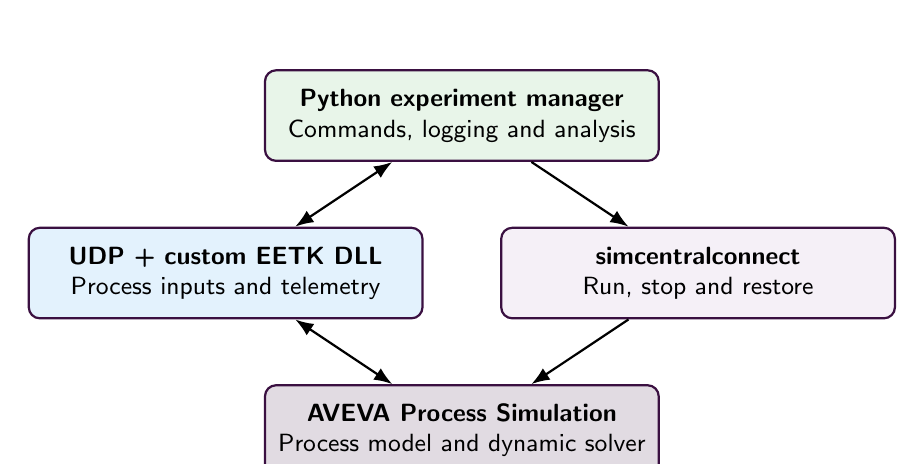
\begin{tikzpicture}[
 block/.style={rectangle,rounded corners,draw=avevaPurple,thick,
 minimum width=5cm,minimum height=1.15cm,align=center,font=\small},
 arrow/.style={->,thick,>=Latex}]
\node[block,fill=tipBg] (py) at (0,0) {\textbf{Python experiment manager}\\Commands, logging and analysis};
\node[block,fill=noteBg] (udp) at (-3,-2) {\textbf{UDP + custom EETK DLL}\\Process inputs and telemetry};
\node[block,fill=avevaLight] (api) at (3,-2) {\textbf{simcentralconnect}\\Run, stop and restore};
\node[block,fill=avevaPurple!15] (aps) at (0,-4) {\textbf{AVEVA Process Simulation}\\Process model and dynamic solver};
\draw[arrow,<->] (py) -- (udp);
\draw[arrow] (py) -- (api);
\draw[arrow,<->] (udp) -- (aps);
\draw[arrow] (api) -- (aps);
\end{tikzpicture}
\vfill
{\large\textbf{Ezequiel Jos\'{e} Valencia Urbina}\par}
{\normalsize Mechatronics Engineer\\M.Sc. Candidate -- Mechanical Systems Dynamics\\University of Bras\'{i}lia (UnB), Brazil\par}
\vspace{0.3cm}
\texttt{urbina.ezequiel@aluno.unb.br}\par
\vspace{0.4cm}
{\small September 2026 -- Revised integration workflow\par}
{\color{avevaPurple}\rule{\textwidth}{1.5pt}}
\end{titlepage}
\tableofcontents
\newpage

\section{Introduction and System Architecture}
This guide explains how to combine a custom UDP bridge with the official \texttt{simcentralconnect} scripting interface to automate dynamic experiments in AVEVA Process Simulation (APS). The same architecture can support tank systems, valve examples and other process models after their variables, units and operating constraints have been defined.

The custom DLL connects external commands to the process equations and exports measurements. Python uses UDP for this data exchange and \texttt{simcentralconnect} to manage the simulation lifecycle. APS remains responsible for solving the process dynamics; this workflow does not require reimplementing the process differential equations in Python.

\subsection{Responsibilities of Each Component}
\begin{tabularx}{\textwidth}{l X}
\toprule
\textbf{Component} & \textbf{Responsibility} \\
\midrule
APS model & Equipment equations, physical constraints and dynamic state evolution. \\
Custom EETK DLL & Model-variable binding, command application and telemetry serialization. \\
UDP & Transport of commands and measurements between the DLL and Python. \\
\texttt{simcentralconnect} & Open the simulation, inspect its mode, run dynamics, stop the solver and restore snapshots. \\
Python experiment manager & Select inputs, coordinate experiments, collect results and perform analysis. \\
\bottomrule
\end{tabularx}

\begin{notebox}
UDP does not automatically start, pause or accelerate APS. In this workflow, those execution responsibilities belong to the scripting interface and the simulator settings. UDP carries the process data. Faster-than-real-time execution is possible, but its speed depends on the model, solver configuration and computer.
\end{notebox}

\subsection{Scope and Evidence}
The four-tank experiment supplied with this workflow successfully combined a UDP command with \texttt{RunDynamics}, received telemetry through a simulation time of 20 seconds, and restored the base snapshot. That result demonstrates an operational communication path for the tested case. It does not establish lossless telemetry, exact command-application timing, or compatibility with every APS installation.

The DLL descriptions below are implementation guidance. The exact interface signatures, registration classes and required methods must come from the EETK project that builds against the installed APS version. No abbreviated listing in this guide should be treated as a complete, compilable DLL.

\section{Phase 1: Define the Variables and Communication Contract}
Before editing the DLL, identify the manipulated inputs, measured outputs, relevant states and simulation clock. Record each variable's APS path, data type, units, permitted range and direction of communication.

\subsection{Four-Tank Example}
\begin{tabularx}{\textwidth}{l l l X}
\toprule
\textbf{JSON key} & \textbf{APS variable} & \textbf{Unit} & \textbf{Direction} \\
\midrule
\texttt{q1} & \texttt{Srcs1.Q\_total\_1} & kg/s & Python to APS \\
\texttt{q2} & \texttt{Srcs1.Q\_total\_2} & kg/s & Python to APS \\
\texttt{h1} & \texttt{T1.LHeight} & m & APS to Python \\
\texttt{h2} & \texttt{T2.LHeight} & m & APS to Python \\
\texttt{h3} & \texttt{T3.LHeight} & m & APS to Python \\
\texttt{h4} & \texttt{T4.LHeight} & m & APS to Python \\
\texttt{sim\_time} & Clock binding to verify & s & APS to Python \\
\bottomrule
\end{tabularx}

The tested configuration uses localhost, with Python receiving on port 5005 and the DLL receiving commands on port 5006. Preserve these settings when reproducing that experiment. Assign a different port pair to each simultaneous simulation instance.

\begin{lstlisting}[style=pythonstyle,caption={Existing four-tank message format: UTF-8 JSON}]
# Python -> DLL, destination 127.0.0.1:5006
{"q1": 0.08, "q2": 0.05}

# DLL -> Python, destination 127.0.0.1:5005
{"sim_time": 20.0, "h1": 0.1805, "h2": 0.1725,
 "h3": 0.0747, "h4": 0.0782}
\end{lstlisting}

For a valve example, replace the input contract with the valve opening and the output contract with flow and actual opening. If an existing valve DLL accepts a plain numeric string, its Python sender must use that format. Changing to JSON requires modifying both ends.

\subsection{Recommended Protocol Extensions}
For repeatable automated experiments, extend the protocol with a run identifier, command identifier, telemetry sequence number and measured applied inputs. These fields are proposed additions; they were not present in the demonstrated four-tank packets. A successful UDP send only confirms local transmission, not receipt or application inside APS.

Specify how invalid commands, out-of-range values and missing updates are handled. Validate finite numeric values and apply multi-input commands atomically. Record any rejected command rather than silently changing its meaning.

\section{Phase 2: Create or Adapt the EETK DLL}
\subsection{Start from a Compatible Project}
Use the existing working DLL project or copy an official EETK example supplied for the installed APS version. Build the unchanged example first. Preserve its required interface methods, registration mechanism and lifecycle structure while adding process-specific behavior.

Check the target framework, process architecture and referenced assemblies against that working project. Installation directories and assembly names vary; use the paths actually present on the computer. A project can reside outside the SDK directory if its references and build paths are configured correctly.

\subsection{Bind Inputs and Measurements}
Declare the variables required by the selected process. For the four-tank example, the bridge needs two commanded inlet flows, four measured levels and access to the simulation clock. Additional signals may be needed to verify applied commands or process constraints.

A residual-based input constraint can be written as
\begin{equation}
r_i = u_{i,\mathrm{APS}} - u_{i,\mathrm{command}} = 0.
\end{equation}
Its derivative with respect to the corresponding APS input is one when the held command is independent of the solver variables. The complete model must have a consistent specification and equation count. Release only the specification that the external equation replaces; measurement bindings do not provide additional physical closure equations.

\begin{notebox}
Declare equation dependencies and derivatives according to the installed EETK contract. Adding every measured variable to every incidence row is not a general remedy for singularity. Check actual dependencies, missing equations, duplicate constraints and the toolkit's rules for exposing read-only measurements.
\end{notebox}

\subsection{Separate Network Handling from Equation Evaluation}
Initialize sockets once within an appropriate object lifecycle and close them when the bridge is disposed. Use nonblocking I/O or a dedicated network worker so that equation evaluation never waits for a UDP packet. UDP sockets can block unless explicitly configured otherwise.

The network worker should parse a complete command and publish it to a synchronized buffer. Model access and command acceptance must occur through supported EETK mechanisms. Hold the accepted command constant throughout the relevant numerical evaluation; changing it between residual or Jacobian evaluations can make the numerical problem inconsistent.

\begin{lstlisting}[style=csharpstyle,caption={Conceptual DLL design; adapt to the installed EETK interface}]
// Initialization:
//   Bind the command socket and define the telemetry destination.
//   Initialize a complete command and its validity information.
//
// Network worker:
//   Receive, parse and validate a complete input vector.
//   Publish it to a synchronized pending-command buffer.
//
// Supported model synchronization point:
//   Accept the pending command as a held input vector.
//
// Equation evaluation:
//   Compute residuals and derivatives using the held vector.
//   Do not wait for network I/O or modify model state from a worker.
//
// Telemetry:
//   Publish time, observations and command identity when available.
//
// Reset/disposal:
//   Clear stale commands; stop workers; release sockets.
\end{lstlisting}

\subsection{Telemetry and Solver Iterations}
Prefer telemetry associated with accepted integration states when the interface provides such a hook. If the existing bridge transmits during residual evaluation, classify those packets as solver observations. They may include repeated timestamps, intermediate iterates or rejected trial states.

Testing \texttt{calculateDerivative == false} alone does not prove that a sample is an accepted integration step. Likewise, sending only on the last equation does not guarantee one packet per timestep. Preserve raw packets and validate the endpoint separately.

Use locale-independent serialization, explicit units and sufficient precision for the intended analysis. A value displayed to four decimal places in metres can conceal smaller level changes.

\section{Phase 3: Configure and Validate the APS Model}
\begin{enumerate}[leftmargin=1.5em,itemsep=0.4em]
\item Build the adapted DLL and deploy it using the add-on loading procedure for the installed APS version. Ensure the process releases the old assembly before replacing a loaded build.
\item Create or adapt the external model block. Match its variables, implementation class and bindings to the actual DLL project.
\item Connect manipulated variables and measurement aliases to the physical process. Check units and eliminate conflicting specifications.
\item Verify a consistent base solution, configure Dynamics mode, and create a named snapshot containing the intended initial condition.
\item Test a small input change. Confirm the actual manipulated variable changes and the resulting outputs respond consistently.
\item Stop and restore the snapshot. Confirm the initial conditions and clock behavior before repeating the experiment.
\end{enumerate}

For the demonstrated setup, the simulation name was \texttt{Sim 3} and the snapshot was \texttt{start dym}. These are configuration values, not universal APS names.

\begin{notebox}
A snapshot may restore the simulator state without restoring private DLL fields, pending UDP messages or external controller memory. Define a separate bridge-reset procedure and verify its behavior. Restoring only the four reported tank levels is not automatically equivalent to restoring the complete dynamic state.
\end{notebox}

\section{Phase 4: Coordinate Python, UDP and simcentralconnect}
\subsection{Python Project Organization}
A reusable implementation can separate responsibilities into \texttt{aveva\_engine.py} for lifecycle calls, \texttt{udp\_bridge.py} for communication, and \texttt{run\_experiment.py} for the experiment sequence. Store configuration and result files alongside the project in clearly named directories.

Use the Python environment in which \texttt{simcentralconnect} already connects successfully. Check compatibility before changing the interpreter or installing analysis dependencies. The custom EETK DLL runs inside APS; Python communicates with it through UDP rather than loading that DLL directly.

\subsection{Known Lifecycle Calls}
The following excerpt uses method names observed in the supplied APS diagnostic. It illustrates lifecycle control only; the UDP acquisition worker and command synchronization must be integrated around it.

\begin{lstlisting}[style=pythonstyle,caption={Lifecycle excerpt based on the demonstrated APS interface}]
import json
import simcentralconnect

SIM_NAME = "Sim 3"
SNAPSHOT_NAME = "start dym"
TIMEOUT_MS = 120000

sc = simcentralconnect.connect().Result
sc.SetOptions(json.dumps({
    "Timeout": TIMEOUT_MS,
    "EnableApiLogging": "false",
}))
sm = sc.GetService("ISimulationManager")
snap = sc.GetService("ISnapshotManager")

def require_success(value, operation):
    if not bool(value):
        raise RuntimeError(f"APS operation failed: {operation}")

require_success(sm.OpenSimulation(SIM_NAME).Result, "open")
require_success(sm.TriggerStopSolve(
    SIM_NAME, TIMEOUT_MS).Result, "stop before reset")
require_success(snap.RevertSnapshot(
    SIM_NAME, SNAPSHOT_NAME, TIMEOUT_MS).Result, "restore")

mode = str(sm.GetSimulationMode(SIM_NAME, TIMEOUT_MS).Result)
if mode != "Dynamics":
    raise RuntimeError(f"Expected Dynamics mode; received {mode}")

# Start and confirm the UDP worker before this point.
# Submit the input command using the agreed protocol.
# Check command acceptance when the bridge supports it.
require_success(sm.RunDynamics(
    SIM_NAME, 20.0, "s").Result, "run dynamics")

require_success(sm.TriggerStopSolve(
    SIM_NAME, TIMEOUT_MS).Result, "stop after run")
# Keep acquisition active while pending telemetry is drained.
# Save observations and validate the final simulator state.
require_success(snap.RevertSnapshot(
    SIM_NAME, SNAPSHOT_NAME, TIMEOUT_MS).Result, "final restore")
\end{lstlisting}

Production code must attempt stop and restoration in cleanup handling even when the experiment fails. Report cleanup failures separately and preserve the original error traceback. Shut down the acquisition worker and close sockets on every exit path.

\subsection{Receive While the Simulator Runs}
A blocking \texttt{.Result} call can occupy the experiment process while APS produces telemetry faster than wall-clock time. Reading the socket only after execution can overflow its buffer. A larger receive buffer alone does not guarantee complete data capture.

Use a separate acquisition process for the robust version of this workflow. That process owns the bound UDP socket, continuously receives packets, and streams them to a JSONL file. It can also send commands from the same socket through a small control channel, preserving the source-port behavior of the working test.

On Windows, protect process creation with \texttt{if \_\_name\_\_ == "\_\_main\_\_":}. Import and initialize \texttt{simcentralconnect} only in the parent process. Send small status messages through interprocess queues; do not join a worker while a large undrained queue prevents it from finishing.

\subsection{Distinguish Simulation Time from Wall-Clock Time}
The run argument, API timeout and telemetry clock have different meanings. The demonstrated call reached simulation time 20 seconds from the tested initial condition. Before chaining runs from nonzero times, verify whether the installed \texttt{RunDynamics} method interprets its time argument as a duration or a target time.

Read actual fields from \texttt{GetSimulationTimeDetails}; printing a .NET type name does not reveal the clock value. Record simulation times before and after each run. Use a monotonic Python timer separately to measure computational runtime.

\section{Phase 5: Execute a Repeatable Experiment}
\begin{enumerate}[leftmargin=1.5em,itemsep=0.4em]
\item Open the configured simulation and stop any active solver run.
\item Restore the selected snapshot and verify the initial condition and mode.
\item Reset bridge command state and remove stale telemetry from the previous experiment.
\item Start acquisition and wait until Python confirms the receive socket is ready.
\item Send the complete input vector. Verify acceptance through the implemented protocol or an appropriate actual-input measurement.
\item Advance APS using the validated time semantics while the acquisition process continues receiving.
\item Stop execution, collect pending packets and verify the final simulation time and outputs.
\item Save raw telemetry, endpoint results and experiment metadata.
\item Stop the worker, release its socket and restore the base case as appropriate for the experiment.
\end{enumerate}

If commands are consumed only while the solver executes, an acknowledgement cannot necessarily arrive while APS is paused. Establish that behavior explicitly and record the actual application time; do not wait indefinitely for an unsupported paused-state acknowledgement.

\section{Results, Validation and Troubleshooting}
\subsection{What to Save}
Keep the raw JSONL telemetry and a compact result table. Each experiment should record its identifier, snapshot, requested inputs, verified applied inputs when available, initial and final simulation times, endpoint outputs, packet counts and validity status. Also retain the DLL version, Python configuration and relevant solver settings.

The supplied successful test reported 754 valid JSON packets, zero invalid packets, and timestamps from 0.1 to 20.0 seconds. Its wall-clock runtime was approximately 1.59 seconds. These are observations from one test, not a fixed sample rate or performance guarantee. Without sequence numbers, zero invalid packets does not establish zero packet loss.

\subsection{Common Problems}
\begin{description}[leftmargin=0pt,style=nextline]
\item[Only a restoration message appears.]
Confirm the executed file path, entry point and unbuffered console output. Print the full exception traceback before cleanup; successful restoration does not establish that the experiment ran.
\item[The API succeeds but there are no packets.]
Verify that acquisition starts before dynamics, the DLL is loaded in the selected simulation, the port pair matches, and another program has not occupied the receive port.
\item[Inputs do not change.]
Check the wire format, command validation, variable binding, specifications and actual applied input. A UDP send is not application confirmation.
\item[Telemetry has repeated or decreasing timestamps.]
Determine whether it was emitted during solver iterations, after rejected steps, or across a reset. Retain the raw evidence and separate runs before constructing trajectories.
\item[The model becomes singular.]
Inspect equation counts, released specifications, duplicate constraints, physical bindings and declared derivatives. Apply the incidence rules of the installed toolkit.
\item[Results depend on the previous experiment.]
Check snapshot completeness, DLL-held commands, pending socket messages and controller state. Verify the initial state before each independent run.
\end{description}

\section{Extending the Workflow to Dynamic Operability}
The integration layer provides a way to evaluate the APS process model from Python. It does not, by itself, implement the complete operability algorithm or an Opyrability package interface.

For a fixed initial state, running several constant input pairs for 20 seconds produces sampled endpoint outputs under constant commands. Mapping all admissible input sequences over successive intervals is a broader reachability problem.

For a discrete model, write
\begin{equation}
x_{k+1}=\Phi_{\Delta t}(x_k,u_k), \qquad y_k=g(x_k).
\end{equation}
Each branch must start from its own complete retained state. Reverting to the same base snapshot for every branch repeats independent experiments rather than propagating the current reachable set.

A future adapter should restore a branch state, apply an input vector, advance by a verified interval, return the output, and preserve a reproducible reference to the final state. Snapshot creation and restoration are possible building blocks, but their completeness and interaction with DLL state must be tested.

Boundary selection in a two-output projection is an approximation for a system with additional states. Two states can have the same plotted outputs and different future responses. Compare any boundary-pruning method against a small exhaustive calculation before relying on it.

Use the professor's required Opyrability version for the analysis layer and verify its installed function signatures. Match the desired output set to the actual output variables and units. Distinguish sampled points, an estimated geometric region and any calculated operability index.

\section{Reusable Setup Checklist and Resources}
\begin{tabularx}{\textwidth}{c X}
\toprule
\textbf{Done} & \textbf{Check} \\
\midrule
$\square$ & Inputs, outputs, states, clock, units and bounds are documented. \\
$\square$ & The DLL builds against the installed APS/EETK environment. \\
$\square$ & Equations, specifications and process-variable bindings are consistent. \\
$\square$ & Command format, ports and reset behavior agree on both ends. \\
$\square$ & Acquisition starts before execution and runs independently. \\
$\square$ & Run timing and endpoint validation have been tested. \\
$\square$ & Failures retain their traceback and cleanup restores the intended case. \\
$\square$ & Raw data and experiment metadata are saved for reproducibility. \\
\bottomrule
\end{tabularx}

\vspace{0.6cm}
\noindent\textbf{Project repository supplied by the author:}\\
\url{https://github.com/VzequyU/AVEVA-Process-Simulation-UDP}

\vspace{0.3cm}
\noindent\textbf{Tutorial link retained from the supplied template:}\\
\url{https://youtu.be/r88qSzDYIMg}

\vspace{0.3cm}
\noindent\textbf{Contact:} \texttt{urbina.ezequiel@aluno.unb.br}

\begin{notebox}
This revision is based on the supplied template, communication examples and successful APS execution log. Repository links identify the project; they do not certify that its current contents or every installation-specific detail have been independently verified. Consult the installed EETK and scripting examples for exact interface contracts.
\end{notebox}

\newpage
\section{Phase 6: Using Opyrability 2.0 with the APS--UDP Interface}
\label{sec:opyrability2}

This chapter describes how to place an operability analysis layer above the existing APS integration. APS evaluates the physical process, the custom DLL and UDP exchange process data, and \texttt{simcentralconnect} coordinates execution. Opyrability is used to construct and evaluate output regions through a suitable Python model adapter.

The target is the Opyrability 2.0 distribution required for the research project. The examples below reuse \texttt{multimodel\_rep} and \texttt{OI\_eval} from the supplied working script; their compatibility with the required distribution must be checked locally. The online documentation could not be verified during this revision. No dedicated dynamic-funnel API is assumed.

\subsection{Step 1: Verify the Installed Package}
Run the following diagnostic in the same Python environment used for the analysis. Save its output with the experiment configuration.

\begin{lstlisting}[style=pythonstyle,caption={Check package location, installed metadata and function signatures}]
import inspect
from importlib import metadata
import opyrability

print("Imported module:", opyrability.__file__)
try:
    print("Distribution version:", metadata.version("opyrability"))
except metadata.PackageNotFoundError:
    print("No distribution metadata: record the source checkout.")

for name in ("multimodel_rep", "OI_eval"):
    function = getattr(opyrability, name, None)
    if function is None:
        raise RuntimeError(f"Required function is unavailable: {name}")
    print(name, inspect.signature(function))
    print(inspect.getdoc(function))
\end{lstlisting}

If the professor supplied a repository checkout or a specific revision, record its commit identifier and use its examples to establish the expected API. Do not assume that an arbitrary package installation corresponds to that revision. Resolve dependency compatibility before starting a long APS experiment.

\subsection{Step 2: Define AIS, DOS and the Output Variables}
The Available Input Set (AIS) describes permitted manipulated inputs. The Desired Output Set (DOS) describes output requirements. The Achievable Output Set (AOS) depends on the process model, initial condition, time horizon and allowed input trajectories.

For the four-tank example, a two-input, two-output study can use
\begin{equation}
u=(q_1,q_2), \qquad y=(h_1,h_2).
\end{equation}
The remaining levels must still be retained when evaluating or restoring the dynamic state. Choosing two outputs for plotting does not reduce the physical process to two states.

\begin{lstlisting}[style=pythonstyle,caption={Example input grid and externally supplied output requirements}]
import json
import numpy as np

# Example range already exercised in the four-tank experiments.
# Validate this range against the current model constraints.
AIS_BOUNDS = np.array([[0.05, 0.11], [0.05, 0.11]], dtype=float)
RESOLUTION = [3, 3]
OUTPUT_KEYS = ("h1", "h2")

# This file must contain the project's actual level requirements:
# {"h1": [lower_limit_m, upper_limit_m],
#  "h2": [lower_limit_m, upper_limit_m]}
with open("dos_levels_m.json", encoding="utf-8") as stream:
    limits = json.load(stream)
DOS_BOUNDS = np.array([limits[key] for key in OUTPUT_KEYS], dtype=float)
if DOS_BOUNDS.shape != (2, 2) or not np.isfinite(DOS_BOUNDS).all():
    raise ValueError("DOS must contain two finite [lower, upper] pairs.")
if np.any(DOS_BOUNDS[:, 1] <= DOS_BOUNDS[:, 0]):
    raise ValueError("Each DOS interval must have positive width.")
\end{lstlisting}

The previous stationary script used discharge flows \texttt{XV3.W} and \texttt{XV4.W}, in kg/s. Its desired flow limits cannot be reused as level limits in metres. A new choice of outputs requires a matching DOS and explicitly named axes.

\subsection{Step 3: Implement a Deterministic Endpoint Adapter}
Begin with a fixed-horizon map that is straightforward to reproduce:
\begin{equation}
M_{\tau}(u)=g\!\left(\Phi_{\tau}(x_0,u)\right),
\end{equation}
where every evaluation starts from the same verified state $x_0$ and holds $u$ constant over the interval. The adapter must return a finite output vector in the declared order and units.

The lifecycle and UDP implementation should be encapsulated in an experiment runner. The following runner interface is a project design, not a built-in Opyrability or APS function.

\begin{lstlisting}[style=pythonstyle,caption={Adapter contract; runner methods must be implemented in the project}]
def make_endpoint_model(runner, horizon_s, output_keys):
    def model(u):
        u = np.asarray(u, dtype=float).reshape(-1)
        if u.shape != (2,) or not np.isfinite(u).all():
            raise ValueError("Expected two finite input values.")
        if np.any(u < AIS_BOUNDS[:, 0]) or np.any(u > AIS_BOUNDS[:, 1]):
            raise ValueError("Input outside the declared AIS.")

        # Project-defined method, following the earlier workflow:
        # stop -> restore x0 -> reset bridge -> start receiver ->
        # apply u -> advance -> validate endpoint -> save -> cleanup.
        record = runner.evaluate_from_base(
            inputs=u.tolist(), horizon_s=float(horizon_s)
        )
        if not record["valid"]:
            raise RuntimeError(record["failure_reason"])
        y = np.array([record["endpoint"][key] for key in output_keys])
        if not np.isfinite(y).all():
            raise RuntimeError("Non-finite endpoint output.")
        return y
    return model
\end{lstlisting}

The runner must establish validity from the actual endpoint time, command application, state restoration and any required process constraints. Selecting the last UDP packet without checking its meaning is insufficient. A failed run must not be replaced with zero outputs, because that would distort the achievable region.

Evaluate APS sequentially while a single simulation instance is shared. Parallel model calls that change the same simulation, snapshot or socket state can contaminate one another.

\subsection{Step 4: Map a Fixed-Horizon Region and Evaluate Coverage}
After validating the runner and checking the installed function signatures, the call pattern from the existing script becomes:

\begin{lstlisting}[style=pythonstyle,caption={Call pattern inherited from the supplied Opyrability script}]
from opyrability import multimodel_rep, OI_eval

# runner is the validated project-specific APS/UDP experiment runner.
M_20s = make_endpoint_model(runner, 20.0, OUTPUT_KEYS)

region_20s = multimodel_rep(
    M_20s, AIS_BOUNDS, RESOLUTION, plot=False
)
oi_raw = float(OI_eval(region_20s, DOS_BOUNDS))
if not np.isfinite(oi_raw):
    raise RuntimeError("Non-finite operability result.")
print("OI returned by the installed package:", oi_raw)
\end{lstlisting}

Check the package's return convention before labeling the result as a fraction or a percentage. The conceptual percentage coverage for a full-dimensional DOS is
\begin{equation}
OI(\tau)=100\,
\frac{\mu\!\left(AOS(\tau)\cap DOS\right)}{\mu(DOS)},
\qquad \mu(DOS)>0,
\end{equation}
where $\mu$ is area for two selected outputs. Record the actual region-construction method used by the installed package; an interpolated or polytopic region is an estimate based on model evaluations.

A $3\times3$ grid provides a useful communication and workflow check, but it does not establish geometric accuracy. Inspect the output points and refine the grid to assess changes in the region and index. If outputs are collinear, do not invent an area to satisfy a two-dimensional routine.

\begin{notebox}
Label this first result as a \textbf{fixed-horizon, constant-input operability estimate}. Repeating it at several horizons gives a family of endpoint maps. It does not yet reproduce the article's enumeration of changing input sequences.
\end{notebox}

\subsection{Step 5: Construct the Dynamic Funnel}
To reproduce the forward-mapping logic discussed in the article, propagate retained states over successive intervals. Let $U_d$ be the discretized AIS and let $X_0=\{x_0\}$. Then
\begin{align}
X_{k+1} &= \left\{\Phi_{\Delta t}(x,u): x\in X_k,\ u\in U_d\right\},\\
Y_k &= \left\{g(x):x\in X_k\right\}.
\end{align}
Remove trajectories that violate the process constraints under the chosen admissibility definition. If constraints apply continuously, endpoint checks alone are insufficient; intermediate accepted states or simulator event checks are needed.

Every child state needs a reproducible state reference and a link to its parent and input. This can be implemented with validated snapshots or by restoring the base case and replaying the entire stored input sequence. Snapshot reuse requires checking full state and DLL consistency; replay requires deterministic timing and command application and can be computationally expensive.

\begin{lstlisting}[style=pythonstyle,caption={Conceptual propagation algorithm; not a package API}]
frontier = [base_state_reference]
for k in range(number_of_intervals):
    children = []
    for parent in frontier:
        for u in input_grid:
            restore_complete_state(parent)
            synchronize_bridge_with_restored_state()
            apply_command_and_advance(u, delta_t)
            child = validate_and_capture_state(parent, u, k + 1)
            if child.is_admissible:
                children.append(child)
    save_state_nodes_and_outputs(k + 1, children)
    frontier = children  # Exhaustive baseline for a small horizon.
\end{lstlisting}

With 25 input combinations, there are $25^k$ possible input sequences after $k$ intervals before merging or pruning. Start with a short exhaustive calculation to validate state propagation. The simulation lifecycle remains under the APS adapter; region analysis can then use the supported Opyrability representation or a documented geometry conversion.

\subsection{Step 6: Evaluate Boundary-Based Reduction}
The article's exterior-node strategy aims to reduce the number of states propagated. For the four-tank implementation, keep the full stored state associated with every candidate output point before applying a geometric selection rule.

An alpha shape describes the geometry of sampled outputs. It does not establish that interior projected points are irrelevant to future reachability. Different hidden states can share the same $(h_1,h_2)$ coordinates. Consequently, pruning by a two-dimensional boundary must be treated as a tested approximation unless additional model properties justify it.

Compare the reduced method with the short exhaustive baseline using region coverage, missing reachable points, output extrema and computational cost. Record the alpha-shape parameters and any coordinate normalization. If the selected geometry is nonconvex, compute its own area; replacing it with a convex hull can fill unreachable gaps.

\subsection{Step 7: Report Results and Connect to Closed-Loop Work}
For each horizon or interval, save the evaluated points, state references, construction settings, region area, DOS intersection, OI convention and runtime. Keep the DOS fixed when comparing time-dependent coverage. Report whether the sets describe reachability at exactly time $t_k$ or reachability at any time up to $t_k$; the latter is a union of sets and answers a different question.

A nearly constant area alone does not prove convergence of the reachable set or that all trajectories have reached steady state. Check geometry, output extrema, state behavior and sensitivity to the input and time discretization.

For later controller studies, use UDP to exchange measurements and commands at defined simulation-time instants, and use the APS lifecycle interface to coordinate the intervals. Document the controller state and reset it alongside the process. Open-loop reachable coverage describes process potential under the allowed inputs; the performance of a particular controller is a separate result.

\begin{stepbox}{Recommended progression for the four-tank project}
Verify the required Opyrability installation; validate the fixed-horizon adapter; reproduce a small AIS-to-output map; define the level DOS; evaluate and refine its coverage; implement complete-state branching; compare exhaustive and boundary-reduced propagation; then extend the verified workflow to closed-loop experiments.
\end{stepbox}

\end{document}
